\begin{figure}[htbp]
\centering
\begin{tikzpicture}
	\draw (0,0) circle [radius=0.3];
	\draw (0,0) node {1};
	\draw (1,2) circle [radius=0.3];
	\draw (1,2) node {2};
	\draw (2,3) circle [radius=0.3];
	\draw (2,3) node {3};
	\draw (3,2) circle [radius=0.3];
	\draw (3,2) node {4};
	\draw (6,5) circle [radius=0.3];
	\draw (6,5) node {5};
	\draw (6,4) circle [radius=0.3];
	\draw (6,4) node {6};
\end{tikzpicture}

\emph{Se tienen 2 centrales disponibles}

\caption{La entrada del problema, con las 5 ciudades y la cantidad de centrales}
\label{ej_2:ej:entrada}
\end{figure}

\begin{figure}[htbp]
\centering
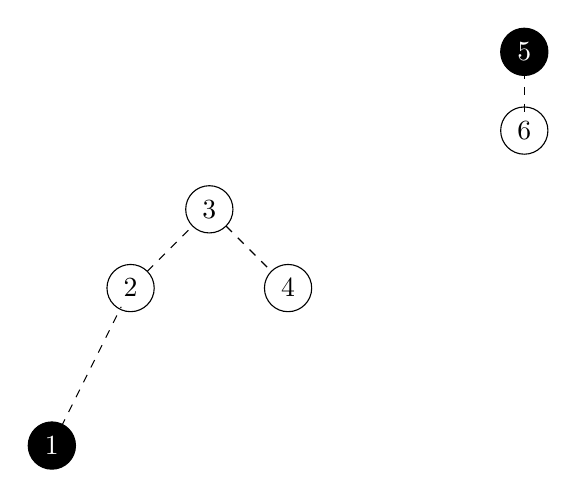
\begin{tikzpicture}
	\draw[fill=black] (0,0) circle [radius=0.3];
	\draw[white] node (v1) at (0,0) {1};
	\draw (1,2) circle [radius=0.3];
	\draw node (v2) at (1,2) {2};
	\draw[style=dashed] (v1) -- (v2);
	\draw (2,3) circle [radius=0.3];
	\draw node (v3) at (2,3) {3};
	\draw[style=dashed] (v2) -- (v3);
	\draw (3,2) circle [radius=0.3];
	\draw node (v4) at (3,2) {4};
	\draw[style=dashed] (v3) -- (v4);
	\draw[fill=black] (6,5) circle [radius=0.3];
	\draw[white] node (v5) at (6,5) {5};
	\draw (6,4) circle [radius=0.3];
	\draw node (v6) at (6,4) {6};
	\draw[style=dashed] (v5) -- (v6);
\end{tikzpicture}
\caption{La soluci\'on al problema de la Figura \ref{ej_2:ej:entrada}, los nodos negros son los que contienen las centrales de distribuci\'on}
\label{ej_2:ej:solucion}
\end{figure}
